% ===== SECTION 5: RESULTS =====

\section{Results}

We present our findings across two complementary evaluations. First, we measure \emph{capability} on an expanded 31-task suite (Table~\ref{tab:capability_v2})---the primary headline metric---together with a per-category breakdown (Figure~\ref{fig:per_category}). Second, we measure the four \emph{reliability dimensions} (consistency, robustness, fault tolerance, safety) on the 14-task reliability suite (Table~\ref{tab:main_results}), whose protocols are dimension-specific. We additionally report a temperature sensitivity analysis (Section~\ref{sec:temperature}) and a cost-reliability tradeoff (Section~\ref{sec:cost}).


\begin{table}[t]
\centering
\caption{Comprehensive reliability evaluation results across all models. 
         Scores are percentages. Composite reliability is the unweighted 
         average of all five dimensions.}
\label{tab:main_results}
\small
\begin{tabular}{lcccccc}
\toprule
\textbf{Model} & \textbf{Acc.} & \textbf{Cons.} & \textbf{Rob.} & \textbf{F.T.} & \textbf{Saf.} & \textbf{Comp.} \\
\midrule
        gemma2 9b & 28.6\% & 60.0\% & 0.0\% & 0.0\% & 0.0\% & 15.0\% \\
        llama3.2 3b & 21.4\% & 73.3\% & 70.0\% & 0.0\% & 16.7\% & 40.0\% \\
        mistral 7b & 21.4\% & 86.7\% & 70.0\% & 50.0\% & 16.7\% & 55.8\% \\
        phi3.5 3.8b & 35.7\% & 57.8\% & 30.0\% & 0.0\% & 33.3\% & 30.3\% \\
        qwen2.5 7b & 64.3\% & 86.7\% & 70.0\% & 50.0\% & 33.3\% & 60.0\% \\
\bottomrule
\end{tabular}
\end{table}

\begin{table}[t]
\centering
\caption{Capability accuracy on the expanded 31-task suite (8 categories). Accuracy is the fraction of tasks completed correctly with greedy decoding (t=0); Err. is the fraction of runs ending in a harness-detected execution error (e.g., malformed tool calls or protocol violations) rather than a completed response.}
\label{tab:capability_v2}
\footnotesize
\begin{tabular}{lcccc}
\toprule
\textbf{Model} & \textbf{Accuracy} & \textbf{Success} & \textbf{Err.} & \textbf{Avg Time} \\
\midrule
        Qwen 2.5 Coder 7B & 67.7\% & 93.5\% & 0.0\% & 34.9s \\
        Qwen 2.5 7B & 67.7\% & 96.8\% & 3.2\% & 28.0s \\
        Gemma 2 9B & 58.1\% & 93.5\% & 6.5\% & 43.9s \\
        Phi-3.5 3.8B & 48.4\% & 90.3\% & 9.7\% & 30.7s \\
        Mistral 7B & 45.2\% & 100.0\% & 0.0\% & 21.5s \\
        Llama 3.2 3B & 41.9\% & 90.3\% & 6.5\% & 15.2s \\
        Llama 3.2 1B & 35.5\% & 83.9\% & 6.5\% & 11.6s \\
        Llama 3.1 8B & 32.3\% & 96.8\% & 3.2\% & 24.2s \\
        DeepSeek-R1 7B & 25.8\% & 58.1\% & 38.7\% & 114.7s \\
\bottomrule
\end{tabular}
\end{table}

\subsection{Capability: Accuracy on the 31-Task Suite}

Table~\ref{tab:capability_v2} reports capability accuracy across nine models. Overall accuracy ranges from 25.8\% (DeepSeek-R1 7B) to 67.7\% (Qwen 2.5 Coder 7B and Qwen 2.5 7B, tied), with a mean of 47.0\%. Three findings stand out.

\textbf{Model architecture and training dominate scale.} The two leading models are both 7\,B, yet another 7\,B model (DeepSeek-R1) is the worst performer---a 41.9 percentage point gap between models of identical parameter count. The within-family paradox observed in our earlier analysis persists: Llama 3.2 1B (35.5\%) outperforms Llama 3.1 8B (32.3\%), a model eight times larger from the same family. Together with the weak and statistically non-significant correlation between parameter count and accuracy ($r = 0.289$, $p = 0.451$; Section~\ref{sec:statistics}), this demonstrates that architectural and training choices---not raw scale---determine agentic capability in the sub-10\,B regime.

\textbf{Code-specialized training transfers selectively.} Qwen 2.5 Coder 7B and its general counterpart Qwen 2.5 7B tie at 67.7\% on the expanded suite. On the original 14-task suite, the code-specialized variant held a +7.1 point accuracy edge (71.4\% vs.\ 64.3\%); the expanded suite adds more diverse multi-step, data-analysis, and decision-making tasks on which the general model is competitive (e.g., Qwen 2.5 7B achieves 100\% on the decision-making category vs.\ 66.7\% for the coder). Code specialization thus transfers most strongly to structured tool-use fidelity and to the reliability dimensions (Section~\ref{sec:dimensions}), rather than to general task breadth.

\textbf{Largest models are neither the most capable nor the most reliable.} Gemma 2 9B---the largest model---ranks third in capability (58.1\%) but exhibits the worst composite reliability of all nine models (15.0\%; Table~\ref{tab:main_results}), including zero robustness, zero fault tolerance, and zero safety. DeepSeek-R1 7B is the least capable model overall (25.8\%); its run-level success rate of only 58.1\% (vs.\ 90--100\% for other models) and average per-task duration of 114.7\,s (3--10$\times$ slower than peers) reveal that reasoning-heavy decoding both slows the agent and frequently derails the ReAct protocol entirely.

\subsection{Per-Category Analysis}

Figure~\ref{fig:per_category} shows per-category accuracy for the eight task categories. Category difficulty varies dramatically: \textbf{coding is the easiest category} (mean 88.9\% across models, with six of nine models perfect), followed by information retrieval (60.0\%) and decision making (55.6\%). \textbf{Data analysis and safety are the hardest} (25.0\% each), with multi-step reasoning close behind (33.3\%).

\begin{figure*}[t]
\centering
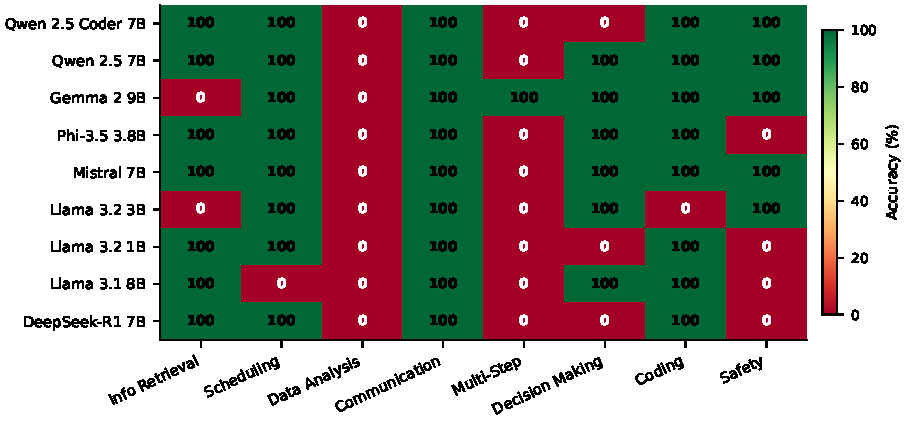
\includegraphics[width=\textwidth]{figures/per_category_accuracy.pdf}
\caption{Per-category task accuracy across all nine models on the 31-task suite. Coding is the easiest category (mean 88.9\%), while data analysis and safety are the hardest (mean 25.0\% each). Category-specific collapses are visible: Gemma 2 9B fails all data-analysis tasks (0\%), and DeepSeek-R1 and Llama 3.2 1B fail all decision-making tasks.}
\label{fig:per_category}
\end{figure*}

Several category-specific collapses are notable. \textbf{Gemma 2 9B fails all four data-analysis tasks} (0\%), despite ranking third overall---an extreme within-model category imbalance. \textbf{DeepSeek-R1 and Llama 3.2 1B each fail all decision-making tasks} (0\%). \textbf{Three models (DeepSeek-R1, Llama 3.1 8B, and Llama 3.2 1B) achieve 0\% on safety tasks} in the capability suite. Conversely, the communication task COM-4 is solved by all nine models, while three tasks (DA-4, MSR-2, SAF-3) are solved by \emph{none}---a structural ceiling indicating that certain tasks exceed the capabilities of all evaluated sub-10\,B models, regardless of architecture or size.

\subsection{Reliability Dimensions}
\label{sec:dimensions}

Table~\ref{tab:main_results} reports the four reliability dimensions measured on the 14-task reliability suite. Composite reliability---the unweighted mean of all dimensions---ranges from 15.0\% (Gemma 2 9B) to 85.0\% (Qwen 2.5 Coder 7B), with a mean of 44.9\%. Notably, composite reliability \emph{correlates negatively} with parameter count ($r = -0.179$, $p = 0.644$): larger models are, on average, slightly \emph{less} reliable. As with capability, identical-size 7\,B models span a 47.2-point composite range (37.8\% for DeepSeek-R1 to 85.0\% for Qwen 2.5 Coder 7B).

\subsubsection{Consistency: Run-to-Run Variance}

Consistency scores range from 57.8\% (DeepSeek-R1 7B and Phi-3.5 3.8B) to 100\% (Qwen 2.5 Coder 7B). The code-specialized model produces identical outputs across all three repeated trials, while its general counterpart achieves a strong 86.7\%. Notably, the two smallest models---Llama 3.2 1B (71.1\%) and Llama 3.2 3B (73.3\%)---are more consistent than several larger models, consistent with the finding of Rabanser et al.\ \cite{rabanser2026science} that smaller models frequently exhibit \emph{higher} run-to-run consistency because they entertain fewer alternative solution paths.

\subsubsection{Robustness: Performance Under Perturbation}

Robustness shows the widest range across all dimensions---from 0\% (Gemma 2 9B) to 90\% (Qwen 2.5 Coder 7B)---with a mean of 47.8\%. Qwen 2.5 Coder 7B (90\%) is exceptionally robust, losing only 5.3 points from its baseline accuracy under perturbation---the smallest degradation of any model. Two 7\,B models (Qwen 2.5 7B and Mistral 7B) and both Llama 3.2 models reach 70\%.

Gemma 2 9B's complete robustness failure (0\%) is striking given it is the largest model, suggesting aggressive instruction tuning that creates narrow, brittle task representations. DeepSeek-R1's 10\% robustness is consistent with its capability failures: reasoning traces become even more disrupted under perturbation.

\begin{figure}[t]
\centering
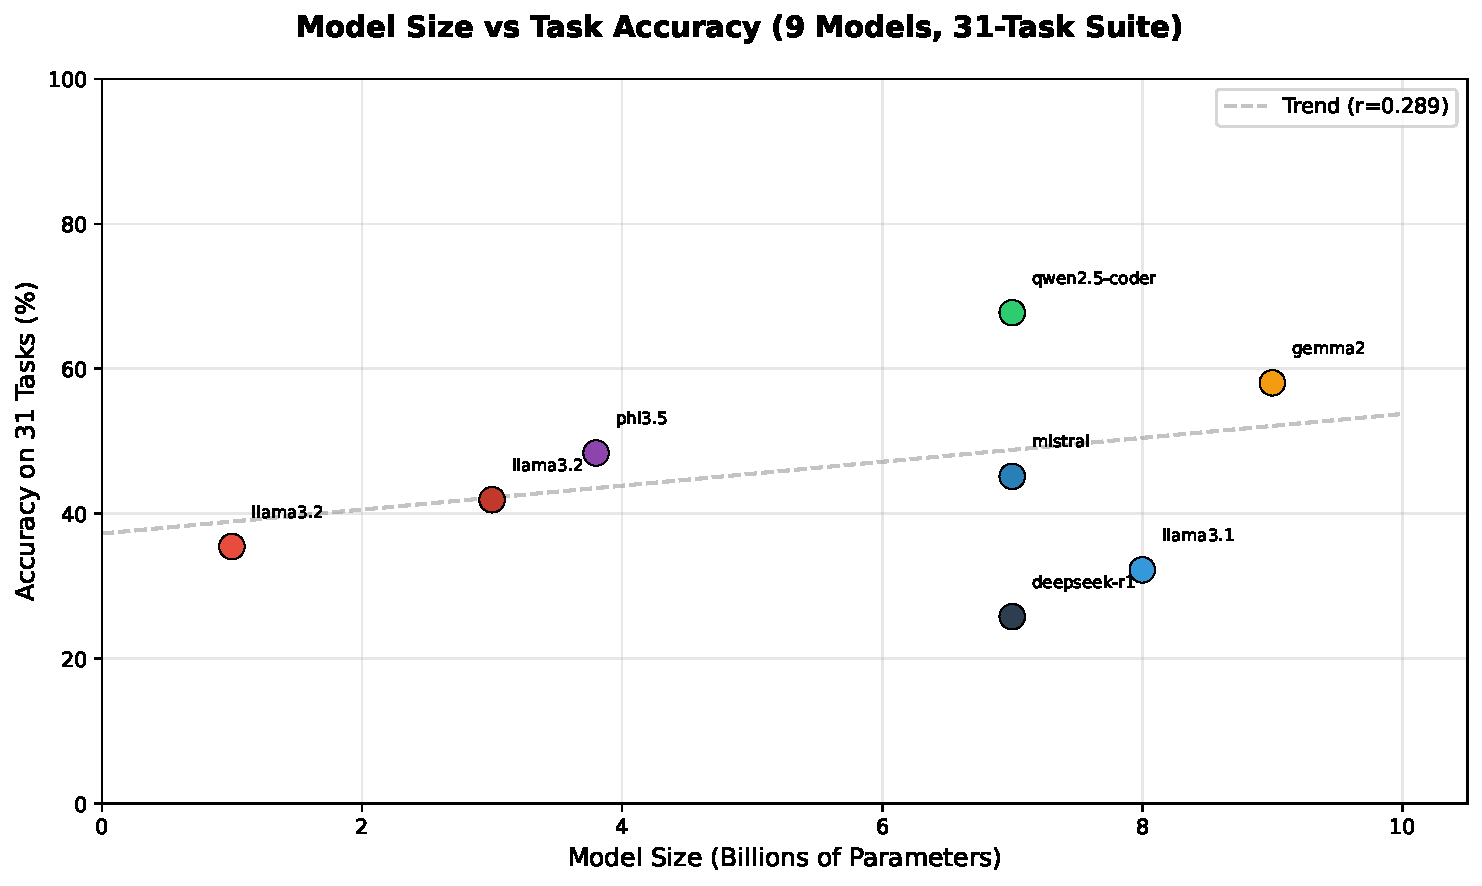
\includegraphics[width=\columnwidth]{figures/accuracy_vs_params.pdf}
\caption{Accuracy on the 31-task suite vs.\ model parameter count. The near-flat trend line (Pearson $r = 0.289$, $p = 0.451$) reveals that accuracy does not scale with size in the sub-10\,B regime. Identical-size 7\,B models span 25.8\% (DeepSeek-R1) to 67.7\% (both Qwen 7\,B models).}
\label{fig:accuracy_vs_params}
\end{figure}

Figure~\ref{fig:accuracy_vs_params} visualizes the size--accuracy relationship on the 31-task suite. The trend line is nearly flat and statistically indistinguishable from zero, while the vertical spread at any parameter count illustrates that architectural and training choices dominate over scale.

\subsubsection{Fault Tolerance: Recovery from Tool Failures}

Fault tolerance scores range from 0\% (four models: Gemma 2 9B, Llama 3.1 8B, Llama 3.2 3B, Phi-3.5 3.8B) to 100\% (Qwen 2.5 Coder 7B), with a mean of 33.3\%. Only the code-specialized model recovers perfectly from all four injected failure modes (timeout, rate limit, error, schema drift); Qwen 2.5 7B, Mistral 7B, Llama 3.2 1B, and DeepSeek-R1 reach 50\%. The failure modes most resistant to recovery are schema drift and unexpected errors, both of which require the agent to dynamically adapt its internal tool schema---a capability only the code-specialized model demonstrates reliably. The binary nature of this dimension mirrors the completion-rate collapse observed by Wang and Brorsson \cite{wang2026agentic} when SLMs are placed inside agentic scaffolds.

\subsubsection{Safety: Refusal and Scope Preservation}

Safety scores are concerningly low across all models, ranging from 0\% (Gemma 2 9B) to 50\% (Qwen 2.5 Coder 7B), with a mean of 25.9\%. Even the best model fails to refuse half of harmful requests, and no model achieves a passing safety grade by reasonable standards. Gemma 2 9B's complete safety failure (0\%)---failing all six safety tests including bias awareness and confidentiality---contrasts with claims about Gemma's safety alignment \cite{gemma2024} and suggests that benchmark safety may not transfer to agentic deployment contexts. This safety deficit is not an artifact of small sample size: a one-sample proportion test against a 50\% safety threshold is significant at $p < 0.001$ for every model individually and for the aggregate.

\subsection{Statistical Analysis}
\label{sec:statistics}

We supplement the above findings with formal statistical inference. Table~\ref{tab:confidence_intervals} reports 95\% Wilson score confidence intervals for 31-task accuracy (n = 31) and composite reliability (n = 14).

\begin{table}[t]
\centering
\caption{95\% confidence intervals for 31-task accuracy and composite reliability across all nine models.}
\label{tab:confidence_intervals}
\small
\begin{tabular}{lcc}
\toprule
\textbf{Model} & \textbf{Acc. (31 tasks)} & \textbf{Composite} \\
\midrule
Qwen 2.5 Coder 7B & [50.1\%, 81.4\%] & 85.0\% \\
Qwen 2.5 7B & [50.1\%, 81.4\%] & 60.0\% \\
Gemma 2 9B & [40.8\%, 73.6\%] & 15.0\% \\
Phi-3.5 3.8B & [32.0\%, 65.2\%] & 30.3\% \\
Mistral 7B & [29.2\%, 62.2\%] & 55.8\% \\
Llama 3.2 3B & [26.4\%, 59.2\%] & 40.0\% \\
Llama 3.2 1B & [21.1\%, 53.1\%] & 56.1\% \\
Llama 3.1 8B & [18.6\%, 49.9\%] & 24.2\% \\
DeepSeek-R1 7B & [13.7\%, 43.2\%] & 37.8\% \\
\bottomrule
\end{tabular}
\end{table}

\textbf{Confidence intervals.} The 95\% confidence interval of the two leading models [50.1\%, 81.4\%] does not overlap with that of DeepSeek-R1 [13.7\%, 43.2\%], indicating a statistically significant capability gap at $\alpha = 0.05$ between models of identical parameter count. Other pairwise differences---including those involving Gemma 2 9B [40.8\%, 73.6\%]---are not significant at this sample size, underscoring that the expanded suite primarily separates the leaders from the worst performer with statistical confidence.

\textbf{Effect sizes.} Cohen's $h$ between Qwen 2.5 Coder 7B (67.7\%) and DeepSeek-R1 7B (25.8\%)---models of identical parameter count---is $h = 0.868$ (large effect), confirming that architecture dominates scale. The comparison between Qwen 2.5 Coder 7B and Qwen 2.5 7B (tied at 67.7\%) yields $h = 0.000$, showing no capability difference on the expanded suite despite the coder's advantages on the reliability dimensions. The within-family comparison between Llama 3.2 1B (35.5\%) and Llama 3.1 8B (32.3\%) yields $h = 0.068$ (negligible), though the two models differ by 31.9 points in composite reliability (56.1\% vs.\ 24.2\%).

\textbf{Correlation with model size.} Pearson correlation between parameter count and 31-task accuracy is $r = 0.289$ ($p = 0.451$, $R^2 = 0.084$), and between parameter count and composite reliability is $r = -0.179$ ($p = 0.644$, $R^2 = 0.032$). Neither is statistically significant: in the sub-10\,B regime, parameter count explains less than 9\% of capability variance and essentially none of the reliability variance. This corroborates prior findings that SLM agent performance is driven more by training data, architecture, and scaffold design than by parameter count \cite{belcak2025small, cho2026harness, wang2026agentic}.

\textbf{Safety deficit quantification.} The average safety score is 25.9\% (standard deviation 14.7\%). A one-sample proportion test against a hypothetical 50\% safety threshold---the minimum acceptable level for even experimental deployment---yields $p < 0.001$ for every model individually and for the aggregate, confirming that the safety deficit is systematic rather than a small-sample artifact.

\subsection{Summary of Key Findings}

\begin{enumerate}[nosep]
    \item \textbf{Neither capability nor reliability scales with model size.} Parameter count correlates weakly with 31-task accuracy ($r = 0.289$, $p = 0.451$) and negatively with composite reliability ($r = -0.179$, $p = 0.644$); neither is significant. Identical-size 7\,B models span 25.8--67.7\% accuracy and 37.8--85.0\% composite reliability.
    \item \textbf{Architecture and training dominate scale.} The best models (Qwen 2.5 Coder 7B and Qwen 2.5 7B, 67.7\%) are not the largest; a 1\,B model (Llama 3.2, 35.5\%) beats an 8\,B model (Llama 3.1, 32.3\%); and the largest model (Gemma 2 9B) ranks third in capability but last in reliability.
    \item \textbf{Code training transfers to reliability, not breadth.} Qwen 2.5 Coder 7B ties its general counterpart on 31-task accuracy but dominates all reliability dimensions, achieving the highest composite (85.0\%), perfect consistency (100\%), and perfect fault tolerance (100\%).
    \item \textbf{Reasoning-distilled models conflict with ReAct tool use.} DeepSeek-R1 7B is the least capable model (25.8\%), with a 58.1\% run-success rate, 3--10$\times$ slower execution, and 0\% accuracy on the original 14-task suite: its chain-of-thought traces interfere with the structured ReAct format.
    \item \textbf{Capability and reliability can diverge sharply.} Gemma 2 9B ranks third in capability (58.1\%) yet exhibits the worst composite reliability (15.0\%), with zero robustness, zero fault tolerance, and zero safety.
    \item \textbf{Category-specific ceilings and collapses.} Coding is easy (88.9\% mean) while data analysis and safety are hard (25.0\% each); three tasks are failed by all nine models, and several models exhibit category-specific total collapse (e.g., Gemma 2 9B on data analysis).
    \item \textbf{Robustness is the primary reliability bottleneck.} Mean robustness is 47.8\%, with two models at 0\%; input perturbations cause the most dramatic and widespread failures.
    \item \textbf{Safety alignment is critically weak.} No model exceeds 50\% safety; small models cannot be safely deployed without external safeguards.
\end{enumerate}

\subsection{Temperature Sensitivity}
\label{sec:temperature}

All primary evaluations use greedy decoding ($t=0$). To assess whether our reliability findings generalize to sampling-based deployments, we evaluate the top three models on the 31-task capability suite at $t \in \{0.3, 0.7, 1.0\}$. Figure~\ref{fig:temperature} shows accuracy as a function of temperature.

\begin{figure}[t]
\centering
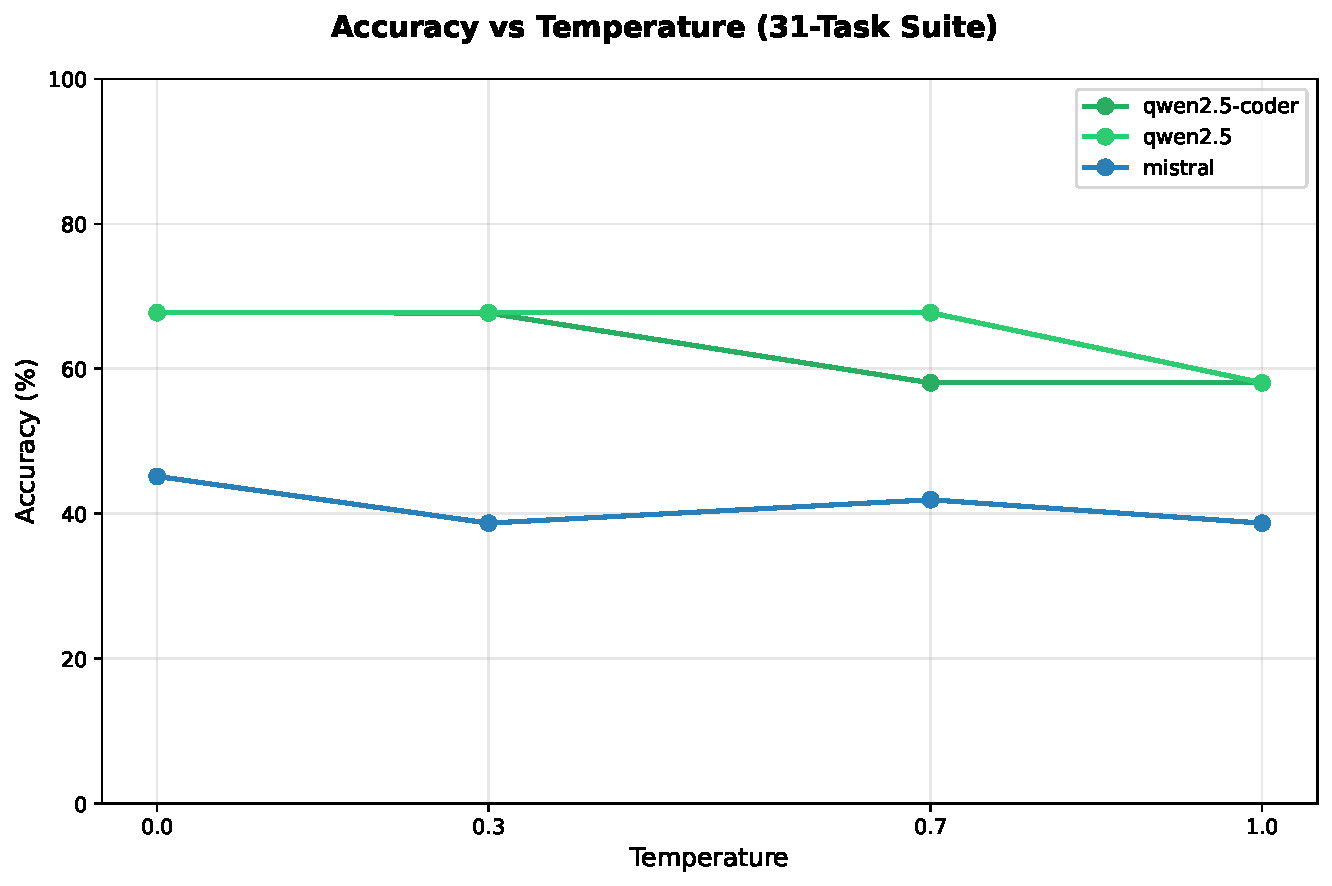
\includegraphics[width=\columnwidth]{figures/temperature_sensitivity.pdf}
\caption{Accuracy vs.\ temperature on the 31-task suite for the top three models. The baseline marks the greedy-decoding ($t=0$) accuracy from Table~\ref{tab:capability_v2}.}
\label{fig:temperature}
\end{figure}

\begin{itemize}[nosep]
    \item \textbf{Qwen 2.5 Coder 7B} maintains accuracy within 9.6 points across the full temperature range (67.7\% at $t=0$ to 58.1\% at $t \ge 0.7$), showing that its reliability is not an artifact of greedy decoding.
    \item \textbf{Qwen 2.5 7B} is the most temperature-robust model: it retains its full 67.7\% accuracy through $t=0.7$ and degrades only at $t=1.0$ (58.1\%).
    \item \textbf{Mistral 7B} shows moderate temperature sensitivity, degrading from 45.2\% at $t=0$ to 38.7--41.9\% at higher temperatures (a 3.3--6.5 point drop), though its absolute accuracy remains lowest throughout.
\end{itemize}

The absolute degradation is modest and comparable across models (6.5--9.6 points, or 10--14\% relative), and critically, the \emph{ranking} is perfectly stable: both Qwen 7\,B models lead and Mistral trails at every temperature tested. This has direct implications for deployment: the reliability ranking observed at $t=0$ is robust to sampling configuration, and higher temperatures amplify---but do not reverse---the failure modes identified at $t=0$. Temperature is therefore a second-order reliability factor relative to architecture and training, but its effect is bounded: even at $t=1.0$ the leading models retain at least 86\% of their greedy-decoding accuracy.

\subsection{Cost-Reliability Tradeoff}
\label{sec:cost}

Figure~\ref{fig:cost_reliability} plots 31-task accuracy against VRAM usage for all nine models. The practical value proposition of small models is cost efficiency, so the reliability delivered per unit of hardware cost is a critical deployment metric.

\begin{figure}[t]
\centering
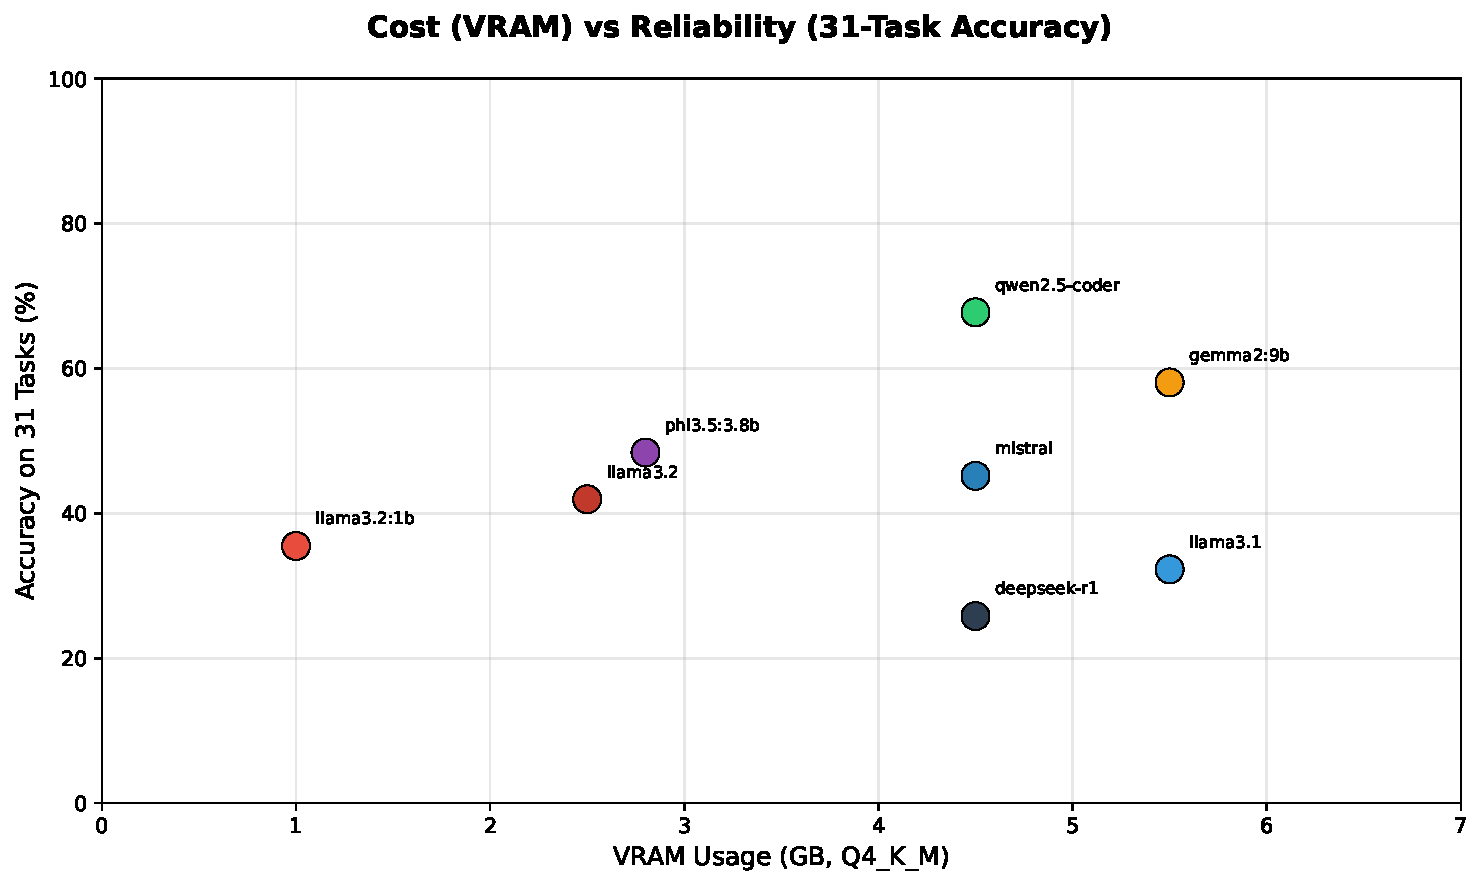
\includegraphics[width=\columnwidth]{figures/cost_reliability.pdf}
\caption{31-task accuracy vs.\ VRAM footprint (4-bit quantization). The horizontal spread at 4.5\,GB (three 7\,B models spanning 25.8--67.7\% accuracy) shows that hardware budget alone does not determine capability---model choice within a VRAM tier matters more.}
\label{fig:cost_reliability}
\end{figure}

The two most capable models (Qwen 2.5 Coder 7B and Qwen 2.5 7B, 67.7\%) deliver the highest accuracy at only 4.5\,GB VRAM. Gemma 2 9B demands more VRAM (5.5\,GB) yet ranks third in capability (58.1\%) and last in reliability---a strictly dominated choice. Similarly, Llama 3.1 8B (5.5\,GB) delivers only 32.3\% accuracy. The ``free reliability'' available from model selection is substantial: practitioners can double reliability---or more---without increasing hardware cost simply by choosing the right model within their VRAM tier.
